\subsection{Surface reconstruction}
\label{ssec:reconstruction}
In \autoref{sec:surfaceBackg} different surface reconstruction schemes have been introduced. In the following we want to discuss our choice for an appropriate surface reconstruction scheme and explain necessary modifications to it.

\subsubsection{Discussion on surface reconstruction schemes}
\tododone[inline]{proofreading Benni\& JC}
Since the surface reconstruction is just an intermediate step before our final \ac{NURBS} fitting procedure, it is not sufficient to only produce a good surface approximation of our optimized topology, but additional constraints have to be kept in mind:
\begin{enumerate}
\item \ac{NURBS} have a rectangular topology, therefore our surface reconstruction should also be able to provide a surface consisting of rectangular patches.
\item Peters' Scheme only covers manifold surfaces, meaning that per edge each patch is only allowed to have exactly one neighbour.
\end{enumerate}
The first requirement is met by \ac{DC}, while the second one is only met by \ac{MC}. We decided to use the \ac{DC} method, because already the basic version of it creates \acp{quad}, while \ac{MC} creates a mesh of triangles, which can only be changed into a mesh of \acp{quad} by considerably increasing the number of faces.

\subsubsection{Our implementation of \ac{DC}}
\tododone[inline]{proofreading Benni\& JC}
We used the open-source language PYTHON \cite{Python} for the implementation of \ac{DC}. Compared to the version described in \cite{Hermite2002} we applied some simplifications:
\begin{itemize}
\item We do not care about sharp features and cannot easily access gradient information in our algorithm. Therefore, we did not use \autoref{eq:QEF} for the generation of new vertices, but the simple averaging scheme described in \autoref{ssec:DC}.
\item For the reason that our dataset only consists of boolean values instead of real valued quantities, we locate our surface at the interface of material and no-material and not at a certain isovalue.
\item We did not implement the adaptive and topology safe scheme but a scheme for uniform grids which does not support adaptive mesh simplification nor topology checks.
\end{itemize}
This leads to the following modified \ac{DC} scheme:
\begin{enumerate}
\item On each cube edge find the root (i.e. the interface of material and no-material voxels) using bisection. We assume our surface to exactly lie in the middle between material and no-material voxels.
\item Take the mean value of all root positions for determining the position of the newly introduced vertex.
\item Join the vertices associated with four cubes sharing a common edge to form a \ac{quad}.
\end{enumerate}
So far our procedure generates \ac{quad} surfaces for boolean datasets on uniform Cartesian grids. But like for the original \ac{DC} algorithm we cannot guarantee that those surfaces are manifold.

\subsubsection{Obtaining manifold surfaces}
%\todointernal[inline]{proofreading!}
Since we want to deduce a first estimate for the topology of the \ac{NURBS} surface output of our \ac{CADTopOpt} tool, non-manifold surfaces cannot be accepted\footnote{Surfaces consisting of smoothly connected \ac{NURBS} \acp{patch} are always manifold surfaces. Therefore we cannot start with a non-manifold surface and assume we will end up with a manifold surface.}. We implemented a remeshing procedure for generating manifold surfaces out of non-manifold surfaces.

Our procedure has the following steps:
\begin{enumerate}
\item Find all non-manifold edges which are connected to more than two \acp{quad}.
\item All non-manifold edges are split into two manifold edges with only two \acp{quad} connected to them.
\item The members of each pair of manifold edges are moved into opposite directions. 
\end{enumerate}
We illustrate the procedure of remeshing for a 2D example in \autoref{fig:manifoldResolution2D}. 
In 3D we do not have non-manifold vertices, but edges, which have to be split and moved. Please note that for the 3D case additional patterns occur. In 3D not only the \acp{quad} which are connected to the whole non-manifold edge have to be considered, but also the \acp{quad} connected to only one vertex of the edge. This also implies the introduction of new \acp{quad} at other locations. For an overview over some of the possible patterns in 3D see \autoref{fig:manifoldPatterns3D}.

\begin{figure}
\begin{center}
\begin{subfigure}[b]{.5\linewidth}
\centering
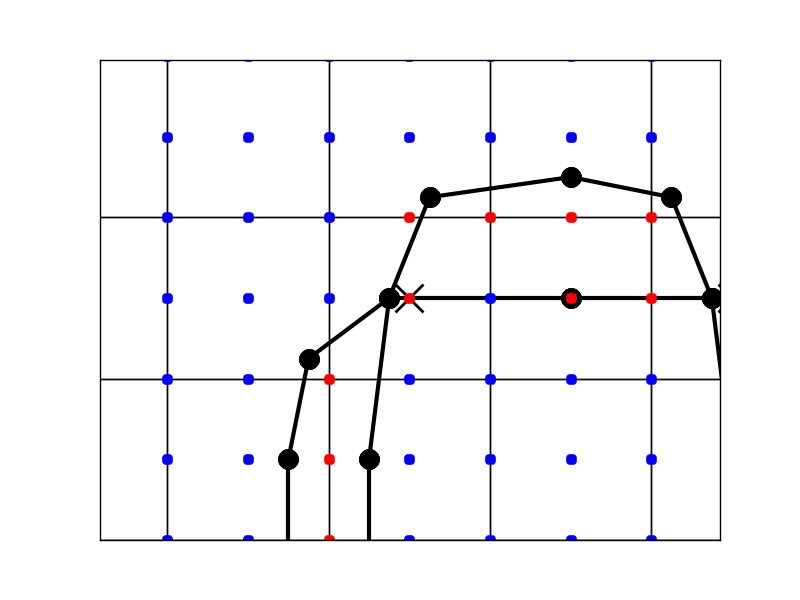
\includegraphics[width = \textwidth]{Pictures/SurfaceReconstruction/2DDoubleTorusNonManifoldDetail}
\subcaption{contour before remeshing}
\end{subfigure}%
\begin{subfigure}[b]{.5\linewidth}
\centering
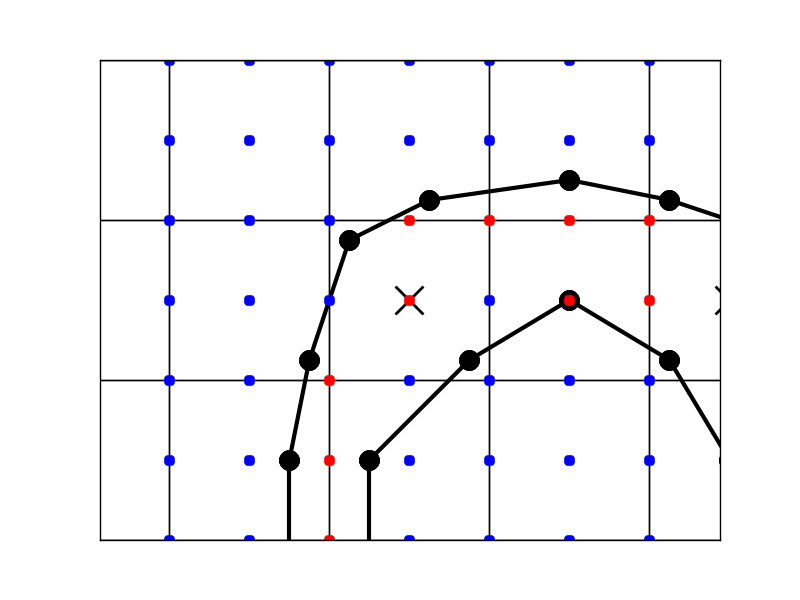
\includegraphics[width = \textwidth]{Pictures/SurfaceReconstruction/2DDoubleTorusManifoldDetail}
\subcaption{contour after remeshing}
\end{subfigure}
\end{center}
\caption{Illustration of the remeshing process. Blue dots denote outside voxels, red dots inside voxels and crosses voxels considered for resolving ambiguities. We first split the non-manifold vertex into two vertices and then move them into opposite directions. The direction is determined from the gradient at the datapoint with the cross, which goes in the direction of the blue dots (from inside to outside). Please note that we can only estimate the gradient if additional information in the middle of the cube, which is containing the non-manifold vertex, is available. Otherwise it is not possible to resolve the ambiguity in a proper way and therefore we cannot eliminate the non-manifold vertex.}
\label{fig:manifoldResolution2D}
\end{figure}

\begin{figure}[p]
\begin{center}
\begin{subfigure}[b]{.45\textwidth}
\centering
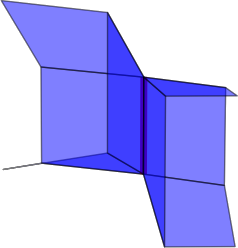
\includegraphics[height = .17\textheight, width = .5\textwidth,keepaspectratio]{Pictures/SurfaceReconstruction/3DManifoldOO}
\end{subfigure}
\begin{subfigure}[b]{.45\textwidth}
\centering
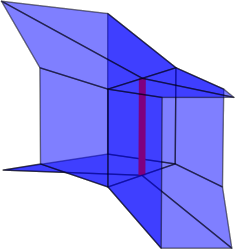
\includegraphics[height = .17\textheight, width = .5\textwidth,keepaspectratio]{Pictures/SurfaceReconstruction/3DManifoldOORes}
\end{subfigure}
\begin{subfigure}[b]{.45\textwidth}
\centering
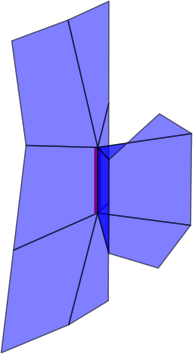
\includegraphics[height = .17\textheight, width = .5\textwidth,keepaspectratio]{Pictures/SurfaceReconstruction/3DManifoldII}
\end{subfigure}
\begin{subfigure}[b]{.45\textwidth}
\centering
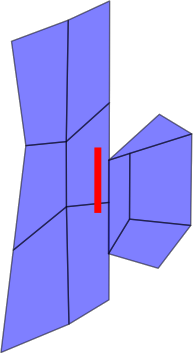
\includegraphics[height = .17\textheight, width = .5\textwidth,keepaspectratio]{Pictures/SurfaceReconstruction/3DManifoldIIRes}
\end{subfigure}
\begin{subfigure}[b]{.45\textwidth}
\centering
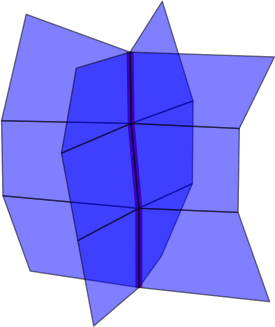
\includegraphics[height = .17\textheight, width = .5\textwidth,keepaspectratio]{Pictures/SurfaceReconstruction/3DManifoldMM}
\end{subfigure}
\begin{subfigure}[b]{.45\textwidth}
\centering
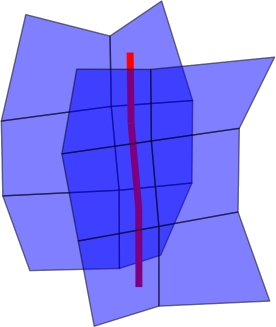
\includegraphics[height = .17\textheight, width = .5\textwidth,keepaspectratio]{Pictures/SurfaceReconstruction/3DManifoldMMRes}
\end{subfigure}
\begin{subfigure}[b]{.45\textwidth}
\centering
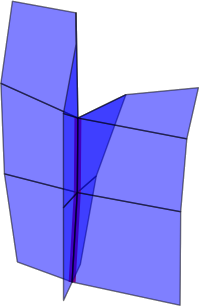
\includegraphics[height = .17\textheight, width = .5\textwidth,keepaspectratio]{Pictures/SurfaceReconstruction/3DManifoldMI}
\end{subfigure}
\begin{subfigure}[b]{.45\textwidth}
\centering
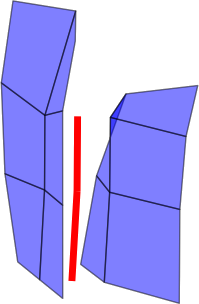
\includegraphics[height = .17\textheight, width = .5\textwidth,keepaspectratio]{Pictures/SurfaceReconstruction/3DManifoldMIRes}
\end{subfigure}
\begin{subfigure}[b]{.45\textwidth}
\centering
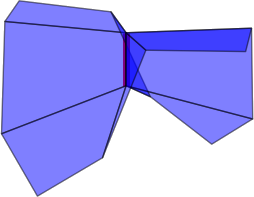
\includegraphics[height = .17\textheight, width = .5\textwidth,keepaspectratio]{Pictures/SurfaceReconstruction/3DManifoldOI}
\end{subfigure}
\begin{subfigure}[b]{.45\textwidth}
\centering
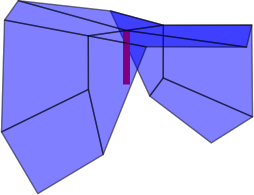
\includegraphics[height = .17\textheight, width = .5\textwidth,keepaspectratio]{Pictures/SurfaceReconstruction/3DManifoldOIRes}
\end{subfigure}
\end{center}
\caption{Different patterns before (left) and after (right) remeshing. Depending on the neighbourhood of the non-manifold edge (red) different patterns are applied. The edge is always divided into to edges which are then moved into different directions. A non-manifold edge is connected to outside-outside (1.row), inside-inside (2.row), two other manifold edges (3.row), inside and another manifold edge (4.row), inside-outside (5.row). In the first and last row just splitting the edge is not sufficient, but additionaly new \acp{quad} have to be introduced. Please note that this figure does not cover all possible patterns.}
\label{fig:manifoldPatterns3D}
\end{figure}







\begin{comment}
\begin{table}
\begin{center}
\begin{tabularx}{.7\textwidth}{|*3{>{\centering\arraybackslash}X}|}
\hline
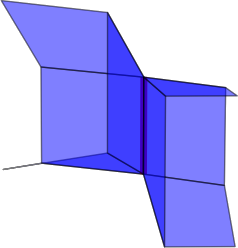
\includegraphics[height=.15\textheight]{Pictures/SurfaceReconstruction/3DManifoldOO}
&
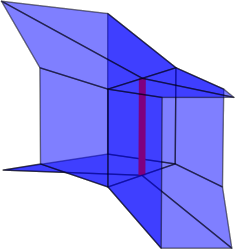
\includegraphics[height=.15\textheight]{Pictures/SurfaceReconstruction/3DManifoldOORes}
\\
\hline
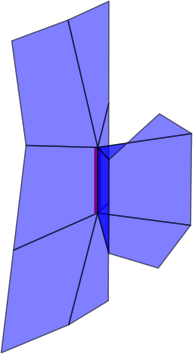
\includegraphics[height=.15\textheight]{Pictures/SurfaceReconstruction/3DManifoldII}
&
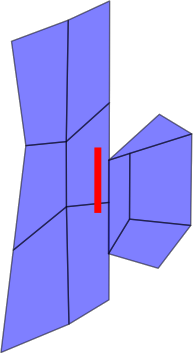
\includegraphics[height=.15\textheight]{Pictures/SurfaceReconstruction/3DManifoldIIRes}
\\
\hline
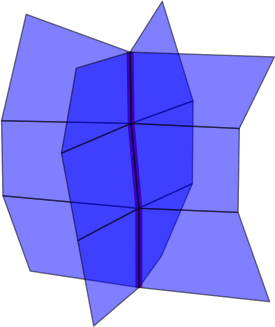
\includegraphics[height=.15\textheight]{Pictures/SurfaceReconstruction/3DManifoldMM}
&
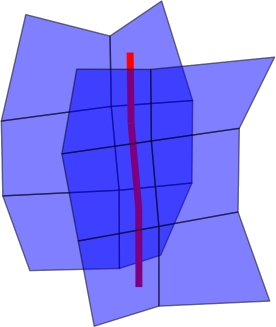
\includegraphics[height=.15\textheight]{Pictures/SurfaceReconstruction/3DManifoldMMRes}
\\
\hline
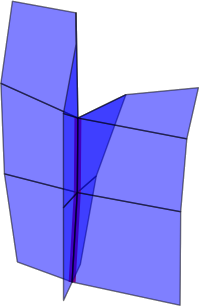
\includegraphics[height=.15\textheight]{Pictures/SurfaceReconstruction/3DManifoldMI}
&
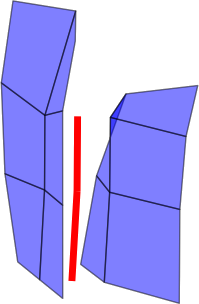
\includegraphics[height=.15\textheight]{Pictures/SurfaceReconstruction/3DManifoldMIRes}
\\
\hline
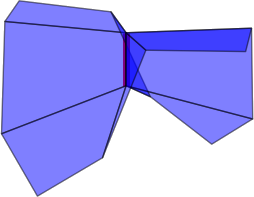
\includegraphics[height=.15\textheight]{Pictures/SurfaceReconstruction/3DManifoldOI}
&
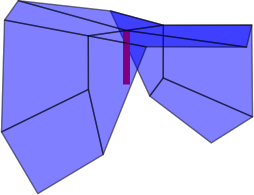
\includegraphics[height=.15\textheight]{Pictures/SurfaceReconstruction/3DManifoldOIRes}
\\
\hline
\end{tabularx}
\end{center}
\end{table}
\end{comment}

\begin{comment}
\begin{figure}[p]
\begin{minipage}[b][.17\textheight]{.45\textwidth}
\begin{center}
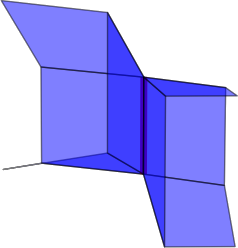
\includegraphics[height=.15\textheight]{Pictures/SurfaceReconstruction/3DManifoldOO}
\end{center}
\end{minipage}
\begin{minipage}[b][.17\textheight]{.45\textwidth}
\begin{center}
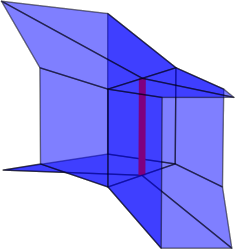
\includegraphics[height=.15\textheight]{Pictures/SurfaceReconstruction/3DManifoldOORes}
\end{center}
\end{minipage}
\begin{minipage}[b][.17\textheight]{.45\textwidth}
\begin{center}
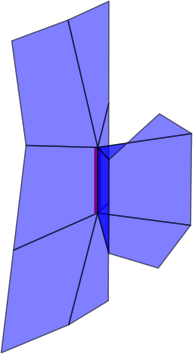
\includegraphics[height=.15\textheight]{Pictures/SurfaceReconstruction/3DManifoldII}
\end{center}
\end{minipage}
\begin{minipage}[b][.17\textheight]{.45\textwidth}
\begin{center}
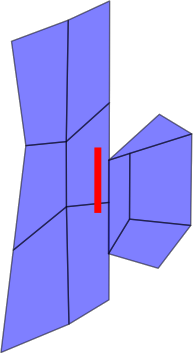
\includegraphics[height=.15\textheight]{Pictures/SurfaceReconstruction/3DManifoldIIRes}
\end{center}
\end{minipage}
\begin{minipage}[b][.17\textheight]{.45\textwidth}
\begin{center}
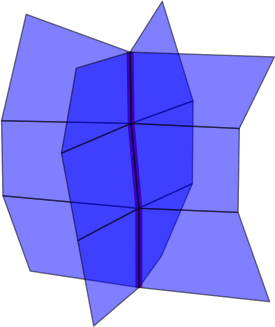
\includegraphics[height=.15\textheight]{Pictures/SurfaceReconstruction/3DManifoldMM}
\end{center}
\end{minipage}
\begin{minipage}[b][.17\textheight]{.45\textwidth}
\begin{center}
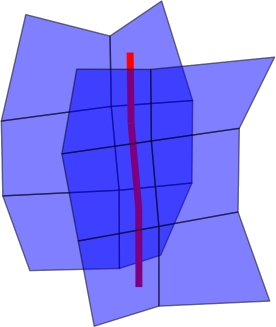
\includegraphics[height=.15\textheight]{Pictures/SurfaceReconstruction/3DManifoldMMRes}
\end{center}
\end{minipage}
\begin{minipage}[b][.17\textheight]{.45\textwidth}
\begin{center}
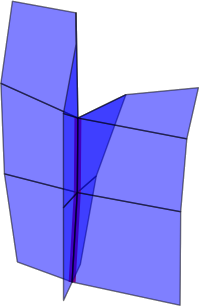
\includegraphics[height=.15\textheight]{Pictures/SurfaceReconstruction/3DManifoldMI}
\end{center}
\end{minipage}
\begin{minipage}[b][.17\textheight]{.45\textwidth}
\begin{center}
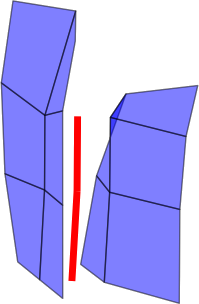
\includegraphics[height=.15\textheight]{Pictures/SurfaceReconstruction/3DManifoldMIRes}
\end{center}
\end{minipage}
\begin{minipage}[b][.17\textheight]{.45\textwidth}
\begin{center}
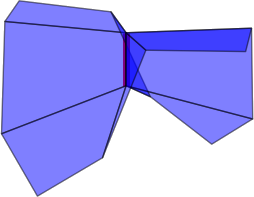
\includegraphics[height=.15\textheight]{Pictures/SurfaceReconstruction/3DManifoldOI}
\end{center}
\end{minipage}
\begin{minipage}[b][.17\textheight]{.45\textwidth}
\begin{center}
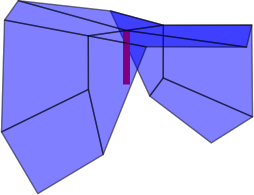
\includegraphics[height=.15\textheight]{Pictures/SurfaceReconstruction/3DManifoldOIRes}
\end{center}
\end{minipage}
\caption{Remeshing schemes for different kinds of manifold edges}
\label{fig:manifoldPatterns3D}
\end{figure}
\end{comment}

\begin{comment}

\subsubsection{Topology--safe adaptivity \ac{DC}}
\todo[inline]{Benni: this is a outlook, remove, put into comment.}
Implementing this feature in \ac{DC} will be one of our major goals in the future. Whether adding adaptivity to the basic \ac{DC} algorithm will destroy the property of \ac{DC} only generating \acp{quad} by introducing \acp{tri}, is going to be part of our future research.

\end{comment}
